% ********** capitulo 5 **********
\chapter{Experimentos y resultados}
\label{sec:chapter5}

En el presente capitulo se describe el conjunto de experimentos realizados
 para evaluar la propuesta planteada ante la problem\'atica de la discapacidad 
 que presentan las personas con problemas de movilidad en los brazos o manos.


%\section{Introducci\'on}

Los algoritmos mostrados en el cap\'itulo \ref{sec:chapter2} proponen formas
 de automatizar actividades realizadas por una persona,   posible 
 implementar ese tipo de soluci\'on al problema en cuesti\'on, pero esto, 
 representar\'ia un problema a\'un mayor, dado que se tendr\'ia que conocer 
 las actividades que realiza el usuario del equipo para poder proponer la 
 automatizaci\'on de \'estas. 


La propuesta planteada en este escrito propone un aprendizaje progresivo,
 discriminando las acciones menos frecuentes realizadas por el usuario y 
 descartando por completo aquellas que no se realizan.

\section{Resultados de experimentaci\'on}

El uso del software no se ve limitado a las personas con movilidad reducida,
 este le puede servir incluso a las personas que no tengan discapacidad 
 alguna, ya que no va por una tarea objetivo espec\'ifica, sino por las 
 actividades que realice la persona de forma frecuente sin importar cuales 
 sean. Con esto en mente, se lograron obtener los archivos con la lista de
 acciones de 7 personas (1 con discapacidad en brazos y manos y 6 sin 
 discapacidades), que realizaban sus actividades cotidianas en sus propios 
 equipos de c\'omputo, esto durante diferentes periodos de tiempo; los primeros 
 cuatro, fueron monitoreados en un plazo de 4 meses; el quinto, 7 d\'ias y los 
 \'ultimos dos, durante 1 mes. 
 
Durante los periodos mencionados las personas tuvieron encendida su 
 computadora diferente cantidad 
 de tiempo el cual se muestra en la segunda columna de la tabla 
 \ref{infodata}. Como ya se explic\'o anteriormente en el cap\'itulo 
 \ref{sec:chapter4} una acci\'on realizada por el usuario genera un nodo, 
 esta cantidad es mostrada en la columna 3, mientras que la columna 4 es el 
 n\'umero m\'aximo de veces que se repiti\'o un nodo y para mantener el 
 anonimato de las personas participantes en esta prueba, se les har\'a 
 referencia por un n\'umero como se muestra en la primer columna. 

Se observa en la tabla \ref{infodata} que el sujeto \textbf{n\'umero 3}
 es el que tiene el mayor tiempo de uso con mas de 1060 horas, con
 1,448,016 nodos generados y 378,541 veces que se repiti\'o un nodo como 
 m\'aximo; mientras que el sujeto \textbf{n\'umero 6} con 1,570,951 nodos, es 
 el que obtuvo mayor cantidad de nodos reportados en 285 horas y 45 minutos 
 con 130,220 repeticiones de un nodo. Esta diferencia en el n\'umero de nodos, 
 se puede deber a la resoluci\'on de la pantalla usado, ya que se monitorea el 
 desplazamiento del rat\'on por pixel, por lo tanto, a mayor resoluci\'on mayor 
 cantidad de pixeles y m\'as nodos por movimientos del rat\'on.
 

\begin{table}[]
\centering
\caption{Informaci\'on de los datos recabados.}
\scalebox{0.9}{
\begin{tabular}{cccc}
\hline
\textbf{No. de Sujeto}	
&   \textbf{Tiempo de Uso (Hr:Min)}		
&	\textbf{N\'umero de Nodos}
&   \textbf{Repeticiones} 	\\   
\hline

1				
&	166:23 						
&	1,494,792			
&	46,036				\\
		
2
&	490:24
&	1,333,016
&	116,001				\\
		
3
&	1060:48
&	1,448,016
&	378,541				\\
		
4
&	148:23
&	972,828
&	56,606				\\ 

5	
&	17:56
&	281,794
&	8,945				\\

6
&	285:45
&	1,570,951
&	130,220				\\

7	
&	37:40
&	418,966
&	23,660				\\
\hline

\end{tabular}
}

\label{infodata}
\end{table}

A cada lista de acciones se le aplic\'o el algoritmo explicado en el
 cap\'itulo \ref{sec:chapter4}, utilizando un factor de 70 incidencias, para 
 que el  nodo 
 sea candidato a formar una secuencia; ya que al utilizar un n\'umero menor, 
 se estar\'ian aceptando la  mayor\'ia de las acciones, lo cual representa un 
 menor tiempo para mostrar una tarea, pero m\'as secuencias basura que 
 tendr\'ia que depurar el usuario  manualmente y por el contrario si el 
 factor es mayor, la identificaci\'on de  secuencias ser\'ia lenta y con 
 algunas secuencias basura, y un m\'inimo de 5  repeticiones por secuencia 
 para declarar que la tarea es \'util. 


Las secuencias de acciones que empieza con la acci\'on \emph{Release} fueron 
 descartadas, ya que esta acci\'on implica que se qued\'o presionada una 
 tecla o bot\'on espec\'ifico; tambi\'en se rechazaron las que 
 terminen con la acci\'on \emph{Pressed} ya que esto dejar\'ia presionada la 
 tecla o bot\'on hasta que se presione f\'isicamente o se mande a llamar la 
 acci\'on \emph{Release}, 
 por ejemplo, una de la tareas que se ver\'ian afectadas por las limitantes
 mencionadas, podr\'ia ser el seleccionar varios iconos no consecutivos en 
 Windows, ya que una forma de hacerlo es mantener presionada(Pressed) la
 tecla CTRL y seleccionar los iconos con el rat\'on uno a uno dando clic 
 sobre ellos y posteriormente soltar(Release) la tecla CTRL, principalmente 
 por la falta de precisi\'on al mover el rat\'on, ya que estas variaciones 
 evitan que se genere una secuencia completa de la tarea, dejando la tecla 
 presionada.

\newpage

En la figura \ref{fig:graphKB}, se presenta el grafo generado con las
 primeras 150 acciones del teclado del sujeto \textbf{n\'umero 3},
 mientras que en la figura \ref{fig:zoomKB} se hace la ampliaci\'on a un
 conjunto de nodos en los que se muestra la relaci\'on de  
 (\textsc{\char13}Keyboard\textsc{\char13},\textsc{\char13}Pressed
 \textsc{\char13},\textsc{\char13}Key.shift\_r\textsc{\char13}) en la parte 
 inferior central y el nodo (\textsc{\char13}Keyboard\textsc{\char13},
 \textsc{\char13}Release\textsc{\char13},\textsc{\char13}Key.shift\_r
 \textsc{\char13}) ubicado en la parte superior izquierda. En la figura 
 \ref{fig:morezKB} se Se muestra el acercamiento al nodo 
 (\textsc{\char13}Keyboard\textsc{\char13},\textsc{\char13}Pressed
 \textsc{\char13},\textsc{\char13}Key.shift\_r\textsc{\char13}),
 en esta se aprecia la relaci\'on con otros nodos, lo cual 
 implica que este nodo, es uno de los que mas se repite, dado que es utilizado
 en varias secuencias usadas por este usuario. 
 
En la siguiente direcci\'on web es posible encontrar el 
 grafo en formato PDF, para su mejor observaci\'on, as\'i como el 
 generado con las primeras 600 acciones del rat\'on por el mismo sujeto.
 
 
\begin{center}
 \url{https://1drv.ms/f/s!Ap61Bj4GJQX2iOppX2n1jChCHyxqdQ} 
\end{center}



\begin{figure}[h]
\centering
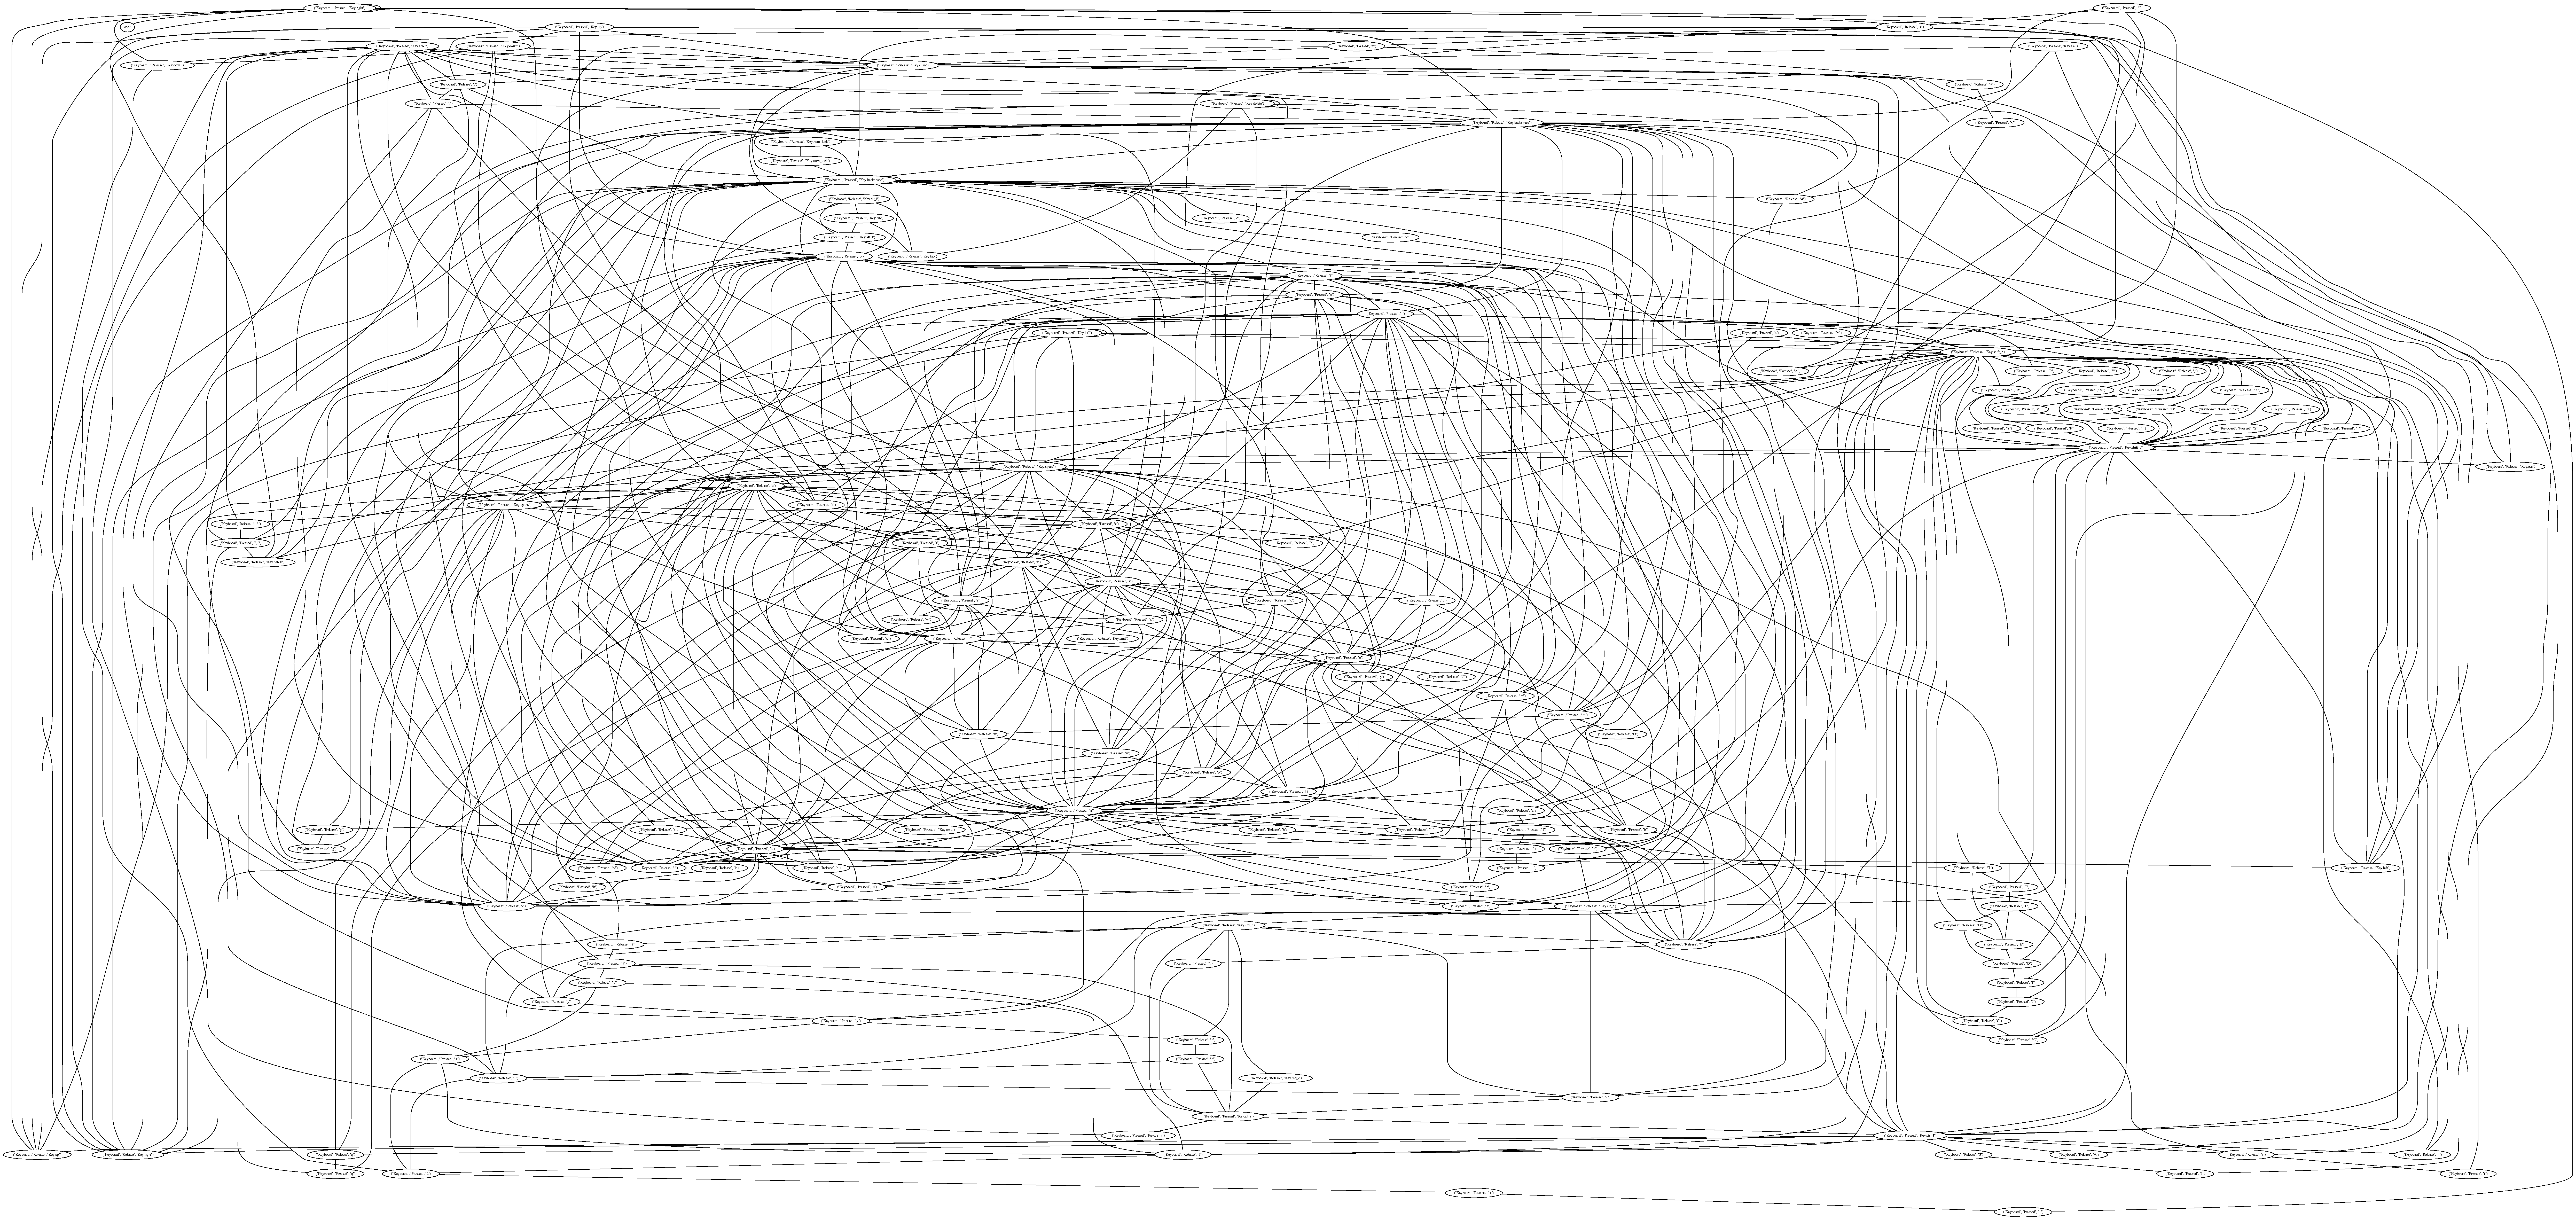
\includegraphics[width=1.0 \columnwidth]{chap5/Imagenes/GraphKB150.eps}
\caption{Grafo generado por el sujeto \emph{n\'umero 3} solo con acciones del 
 teclado.}
\label{fig:graphKB}
\end{figure}



\begin{figure}[h]
\centering
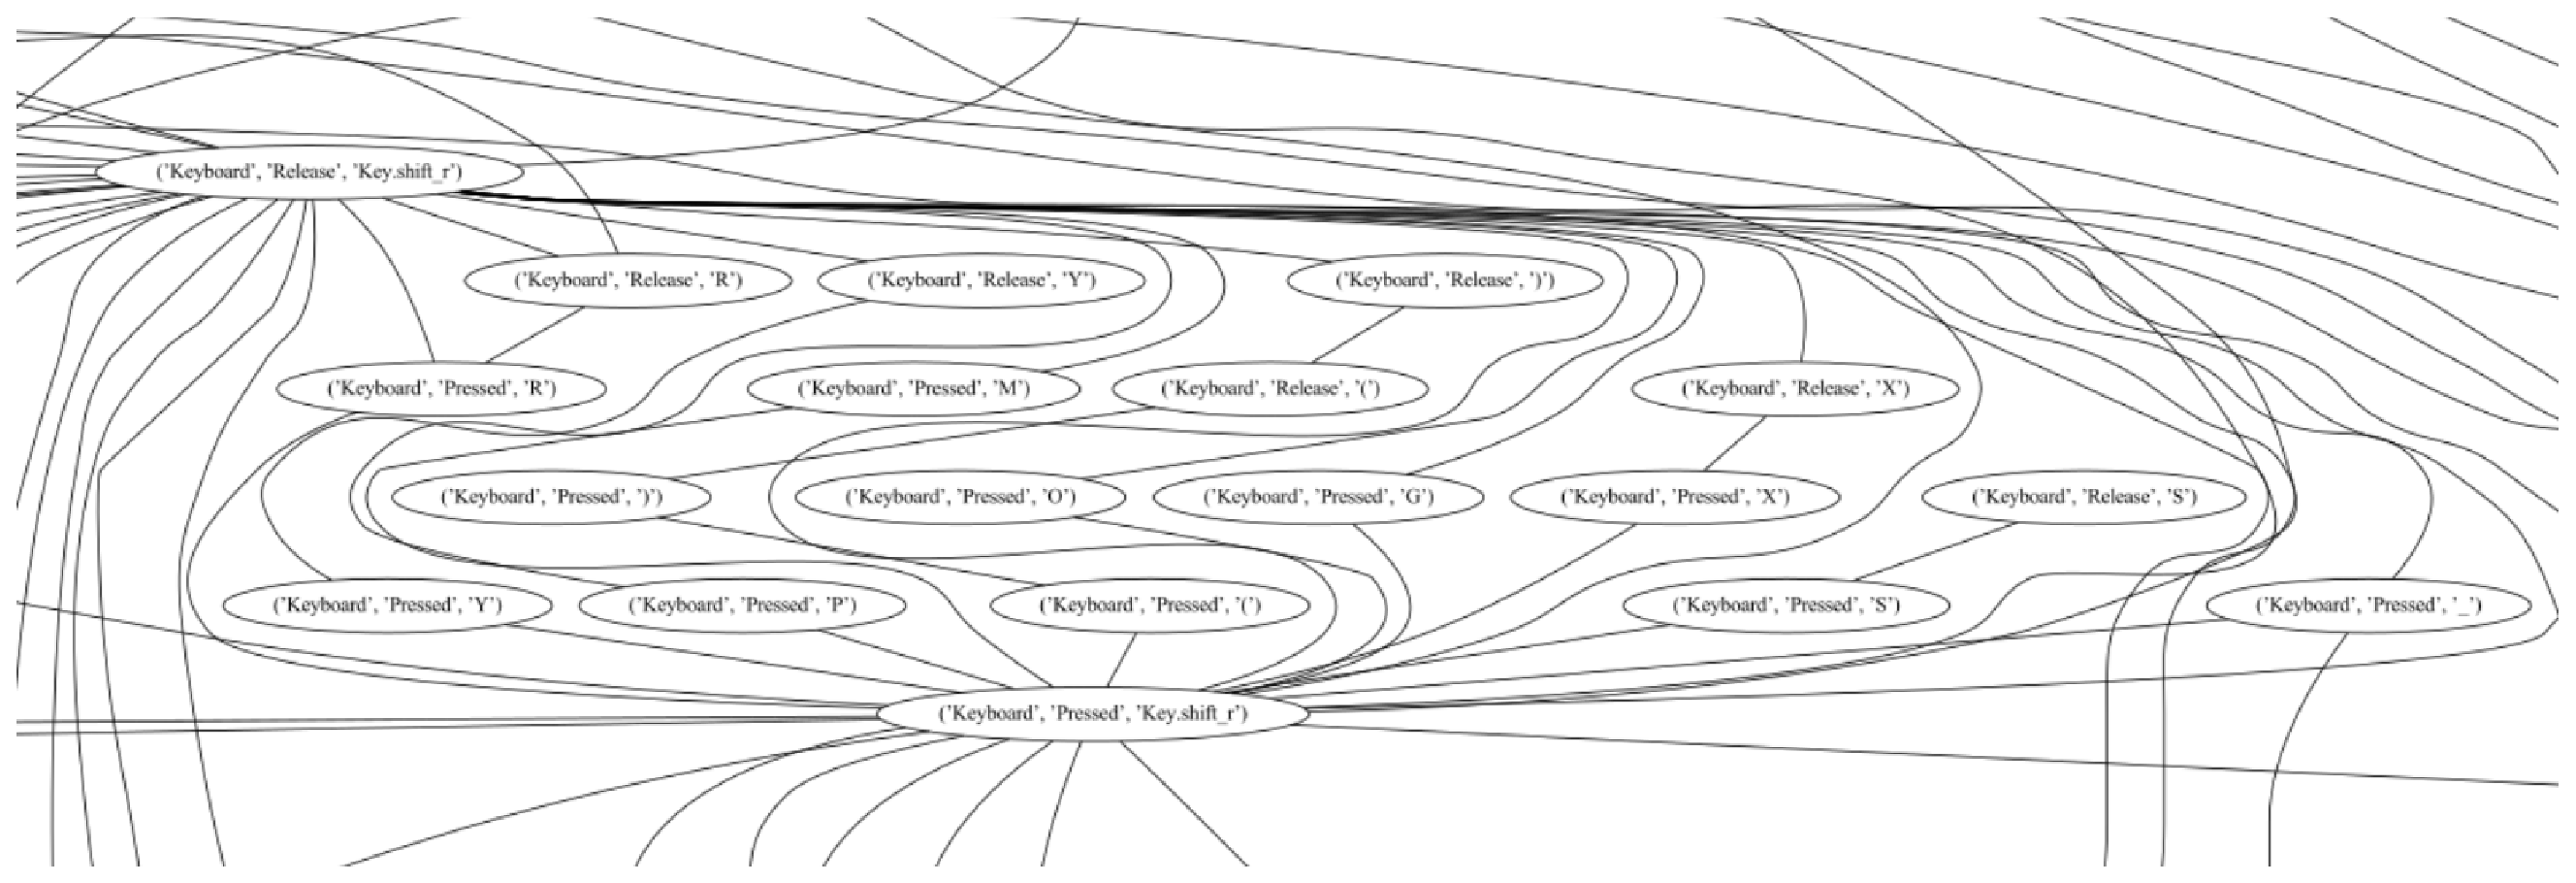
\includegraphics[width=1.0 \columnwidth]{chap5/Imagenes/ZoomKB150.eps}
\caption{Ampliaci\'on al grafo generado por el sujeto \emph{n\'umero 3} solo 
 con acciones del teclado.}
\label{fig:zoomKB}
\end{figure}


\begin{figure}[h]
\centering
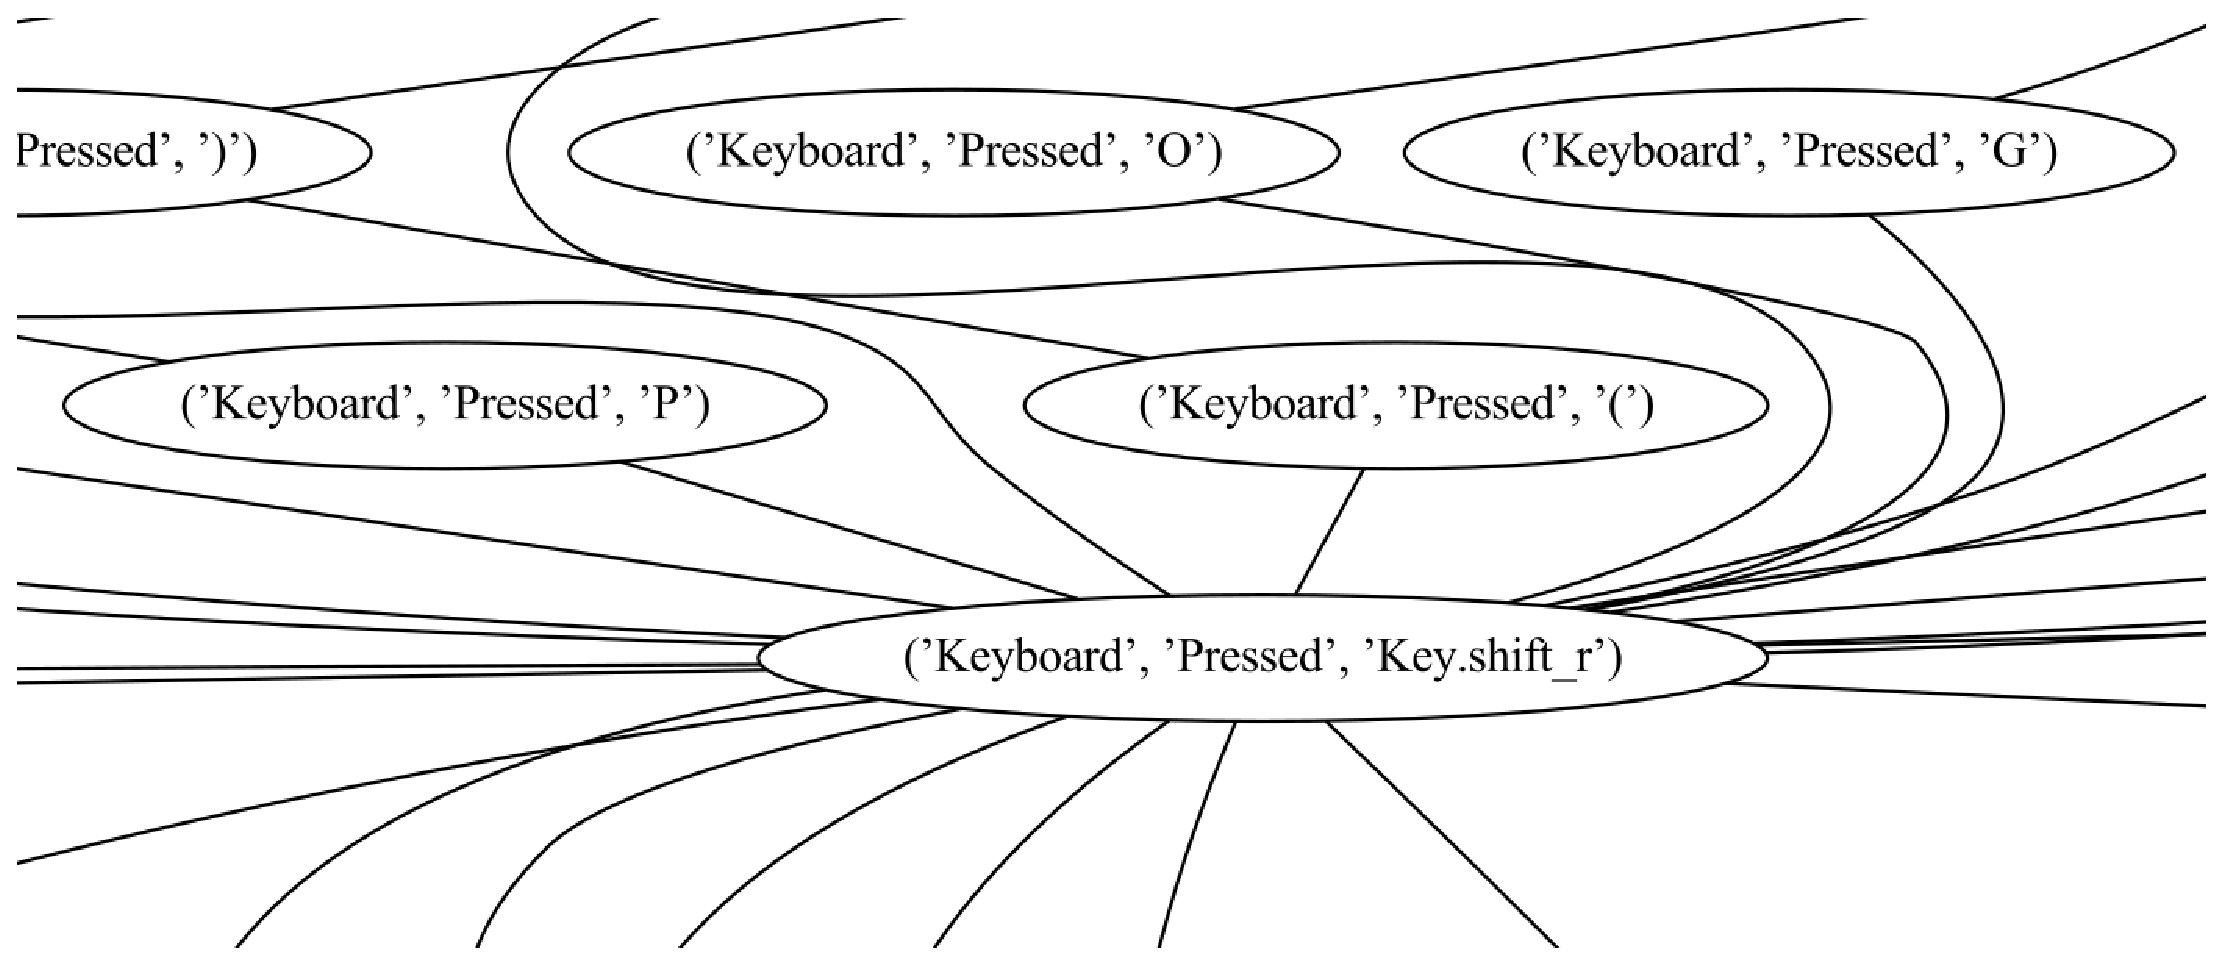
\includegraphics[width=1.0 \columnwidth]{chap5/Imagenes/MoreZKB150.eps}
\caption{Ampliaci\'on para la correcta visualizaci\'on de los nodos en el
 grafo generado por el sujeto \emph{n\'umero 3} solo con acciones del
 teclado.}
\label{fig:morezKB}
\end{figure}


Como filtro adicional, se limit\'o a obtener secuencias de 
 acciones con longitudes en m\'ultiplos de 2, considerando que una tecla o 
 bot\'on presionado debe de ser liberado para concluir la acci\'on, sin 
 embargo, pese a esta limitante, las secuencias a obtener naturalmente son; 
 desde una acci\'on (tabla \ref{tableRes1}) y desde dos acciones (tabla 
 \ref{tableRes2}). 
 

El sujeto \textbf{n\'umero 1} es el que obtuvo mayor n\'umero de 
 \emph{Secuencias Aceptables}, 189 secuencias lo cual corresponde a un 36\% de
 \emph{Porcentaje de Precisi\'on}($P_P$), porcentaje obtenido de la ecuaci\'on 
 \ref{eqAsertividad}, en la que se realiza la divici\'on de las \emph{Secuencias 
 Aceptables} ($S_A$) multiplicadas por $100$ entre el \emph{Total de Secuencias 
 Encontradas} ($S_T$).


\begin{equation}
P_P = \dfrac{ S_A \cdot 100}{S_T}
\label{eqAsertividad}
\end{equation}


El caso contrario es el sujeto \textbf{n\'umero 6}, el cual presenta 43 
 \emph{Secuencias Aceptables} y 28.47\% como \emph{Porcentaje de Precisi\'on}, 
 lo cual se podr\'ia deber a que este uso mayormente el rat\'on, a diferencia 
 del sujeto \textbf{n\'umero 5} (la persona con discapacidad), que obtuvo un 
 \emph{Porcentaje de Precisi\'on} de 35.48\%, pese a ser el usuario que 
 interactu\'o menos tiempo con la computadora (17 horas y 56 minutos), 
 tambi\'en, fue el que obtuvo la menor cantidad de nodos (281,794) y el n\'umero
 m\'as bajo de repeticiones (8,945 repeticiones), ver tabla \ref{infodata}.

 
En la tabla \ref{tableRes2}, se aprecia un incremento en el \emph{Porcentaje de 
 Precisi\'on} con respecto a la tabla \ref{tableRes1}, esto es debido, a la
 eliminaci\'on previa de las acciones unitarias, que por las restricciones 
 establecidas eran rechazadas, lo cual lleva a un incremento considerable en los
 \emph{Porcentajes de Precisi\'on} de los individuos, principalmente, el sujeto
 \textbf{n\'umero 6}, ya que se increment\'o del 28.47\% al 48.71\%. 

\newpage

Por el hecho de que este es un m\'etodo de aprendizaje acumulativo, as\'i sea
 que la primer secuencia sea del agrado del usuario o no, la siguiente 
 secuencia puede contenerla con alguna acci\'on adicional y es mas 
 probable que esta variante, sea de utilidad al usuario. 

 
\begin{table}[]
\centering
\caption{Tabla de resultados con secuencias de una longitud m\'inima de 
 1 acci\'on.}
\begin{tabular}{cccc}
\hline
\textbf{No. de }	
&	\textbf{Secuencias }	
&   \textbf{Secuencias }	
&	\textbf{Porcentaje de }	\\

\textbf{Sujeto}
&	\textbf{Aceptables}
&	\textbf{Totales}
&	\textbf{Precisi\'on}
	\\ \hline

1				
&	189						
&	525						
&	36.00 \%		\\

2				
&	165						
&	487						
&	33.88 \%		\\

3
&	151
&	467
&	32.33 \%		\\

4
&	56
&	180
&	31.11 \%		\\

5
&	55
&	155
&	35.48\%			\\

6
&	43
&	151
&	28.47\%			\\

7
&	66
&	205
&	32.19\%			\\

\hline
\end{tabular}

\label{tableRes1}
\end{table}


\begin{table}[]
\centering
\caption{Tabla de resultados con secuencias de una longitud m\'inima de 
 2 acciones.}
\begin{tabular}{cccc}
\hline
\textbf{No. de }	
&	\textbf{Secuencias }	
&   \textbf{Secuencias }	
&	\textbf{Porcentaje de }	\\

\textbf{Sujeto}
&	\textbf{Aceptables}
&	\textbf{Totales}
&	\textbf{Precisi\'on}
	\\ \hline

1
&	179
&	410
&	43.65 \%		\\
	
2
&	170
&	377
&	45.09 \%		\\

3
&	154
&	346
&	44.50 \%		\\

4
&	52
&	119
&	43.69 \%		\\

5
&	49
&	108
&	45.37\%			\\

6
&	38
&	78
&	48.71\%			\\

7
&	60
&	145
&	41.37\%			\\
\hline
\end{tabular}

\label{tableRes2}
\end{table}

Recapitulando, para que una tarea sea identificable; los nodos que forman la
 secuencia deben de tener un m\'inimo de 75 repeticiones cada uno y cumplir 
 con las restricciones planteadas; no empezar con la acci\'on \emph{Release}, 
 no terminar con la acci\'on \emph{Pressed} y la longitud m\'inima de 
 2 acciones, por lo tanto, las secuencias mostradas a continuaci\'on
 cumplen con estas car\'acter\'isticas:
\\
\\
Sujeto: 1	\\
Descripci\'on: La tarea es utilizada en el software Blender para girar el 
 objeto en el eje Y.	\\
Secuencia obtenida:\\
Keyboard,Pressed,G\\
Keyboard,Release,G\\
Keyboard,Pressed,Y\\
Keyboard,Release,Y\\
\\
Sujeto: 2	\\
Descripci\'on: En Windows es utilizada esta combinaci\'on de teclas para 
 cambiar entre las ventanas abiertas.	\\
Secuencia obtenida:\\
Keyboard,Pressed,Key.alt\_l	\\
Keyboard,Pressed,Key.tab	\\
Keyboard,Release,Key.tab	\\
Keyboard,Release,Key.alt\_l	\\
\\
Sujeto: 3	\\
Descripci\'on: es la palabra ``el''.	\\
Secuencia obtenida:\\
Keyboard,Pressed,e	\\
Keyboard,Release,e	\\
Keyboard,Pressed,l	\\
Keyboard,Release,l	\\
\\
Sujeto: 4	\\
Descripci\'on: En Windows, selecciona el objeto se\~nalado por el puntero y
 obtiene el men\'u contextual de ese objeto.	\\
Secuencia obtenida:\\	
Mouse,Pressed,Button.left	\\
Mouse,Released,Button.left	\\
Mouse,Pressed,Button.right	\\
Mouse,Released,Button.right	\\

\newpage
\section{Discusi\'{o}n de resultados}


Lo m\'as destacable de las pruebas realizadas son los resultados de los sujetos 
 \textbf{n\'umero 5} y \textbf{n\'umero 7}
 (ver tabla \ref{infodata}, \ref{tableRes1} y 
 \ref{tableRes2}) ya que pese a ser los que menos tiempo de uso y
 \emph{Secuencias Totales} obtuvieron, su \emph{Porcentaje de Precisi\'on}
 no var\'ia tanto con respecto al de los dem\'as sujetos, lo cual demuestra 
 una estabilidad en el algoritmo mostrado, considerando que es probable que 
 estos usuarios utilizaron el teclado m\'as que el rat\'on, a diferencia del 
 sujeto \textbf{n\'umero 6}, y tambi\'en es probable que realizaron
 acciones similares cada vez que usaba la computadora, mientras que los 
 dem\'as sujetos tuvieron m\'as diversidad en las acciones realizadas.
 
 
Considerando que los criterios mencionados son para darle un uso espec\'ifico
 al grafo, es destacable que pese al entorno variable en el cual fue evaluado
 el software, solo fue necesario asignar unas pocas
 condiciones generales para obtener las secuencias coherentes. 
 Entre las secuencias rechazadas se pueden localizar tareas que tienen la
 longitud de una acci\'on, las cuales es posible que para alg\'un usuario 
 sean de utilidad, se presenta la siguiente lista a modo de ejemplo.
\\
\\
Secuencia 1:\\
Mouse,Scrolled,Down\\
\\
Secuencia 2:\\
Mouse,Scrolled,Up\\

Cabe recordar que la principal intenci\'on de este software es el apoyar a 
 las personas con discapacidad en brazos y manos, teniendo en cuenta esto, 
 las secuencias de longitud uno, pueden ser de utilidad a alguna persona, sin 
 embargo, considerando que la secuencia m\'as \'util es la que contiene mas 
 elementos, estas acciones unitarias fueron descartadas. Adicionalmente, si 
 se piensa en alg\'un otro uso para el algoritmo, aparte de la 
 automatizaci\'on de las tareas realizadas en una computadora, es posible que 
 las acciones de longitud unitaria tengan importancia, por lo que el
 \emph{Porcentaje de Precisi\'on} mostradas en las tablas \ref{tableRes1} y
 \ref{tableRes2}, puede variar dependiendo del caso de uso.

La lista de tareas obtenida se puede ver incrementada con el uso de estas, por 
 el hecho de que, al hacer uso de las tareas guardadas, el usuario le indica a 
 la maquina que tarea realizar, en lugar de hacerla \'el mismo, est\'e es otro 
 aspecto para destacar ya que solo se crean las secuencias, no se ejecutan 
 autom\'aticamente, si se desea ejecutar alguna tarea guardada, el usuario es
 el que debe ejecutarla manualmente.


Considerando el objetivo a cumplir, el software desarrollado tiene mucha 
 similitud con un creador de macros, por 
 ejemplo, Pulovers Macro Creator, las diferencias que hay que destacar se 
 mencionan en la tabla \ref{vsmacros}, en la que se realiza un an\'alisis 
 comparativo general entre ambos desarrollos. Tambi\'en, existe mucha 
 similitud con el objetivo de la metodolog\'ia de RPA, 
 por lo que en el an\'alisis 
 comparativo entre las metodolog\'ias, presentado en la tabla \ref{vsrpa}, se 
 presentan diferencias destacables entre ambas.
 

\begin{table}[h]
\centering
\caption{An\'alisis comparativo del software con un generador de macros.}
\begin{tabular}{m{6cm}|m{6cm}}
\hline
\textbf{Creador de macros} 	&	\textbf{Software desarrollado} \\
\hline
Hay que indicar manualmente cuando empieza y termina la acci\'on deseada	
 &	
Se monitorea cada acci\'on realizada por el usuario.\\
\hline

El usuario graba manualmente la tarea que desea automatizar	
 &
Se muestra al usuario las acciones que realiza con mayor frecuencia para que
  \'el decida cual guardar\\
\hline

El usuario requiere conocimiento del software para crear tareas complejas 	
 &
El usuario no requiere editar las tareas\\
\hline
\end{tabular}

\label{vsmacros}
\end{table}


\begin{table}[h]
\centering
\caption{An\'alisis comparativo de la propuesta con Robotic Process
 Automation.}
\begin{tabular}{m{6cm}|m{6cm}}
\hline
\textbf{Robotic Process Automation}    &    \textbf{Software desarrollado} \\

\hline
Hay que indicar manualmente cuando empieza y termina la acci\'on deseada.
&
Se monitorea cada acci\'on realizada por el usuario.\\

\hline
Por medio de t\'ecnicas de reconocimiento de im\'agenes y monitoreo a los dispositivos de E/S, se determina la acci\'on realizada y el momento de ejecuci\'on. 
&
Por medio del an\'alisis en tiempo ejecuci\'on de un grafo dirigido se obtienen las tareas realizadas.\\

\hline
Se automatiza un proceso en espec\'ifico.
&
Se automatiza la tarea que m\'as realice el usuario.\\

\hline
\end{tabular}

\label{vsrpa}
\end{table}


Finalmente, la metodolog\'ia desarrollada es una forma autom\'atica de obtener 
 secuencias, se ha observado que, para esta aplicaci\'on, los resultados son 
 prometedores y subjetivos, ya que depende del usuario la definici\'on de las 
 tareas que le puedan ser de utilidad, sin embargo, es posible presentar el 
 proyecto como una forma autom\'atica de realizar la automatizaci\'on de 
 procesos con RPA o de un creador de macros, por medio de aprendizaje 
 autom\'atico.


